\documentclass[11pt]{article}
\makeatletter\if@twocolumn\PassOptionsToPackage{switch}{lineno}\else\fi\makeatother

      \makeatletter
\usepackage{wrapfig}
\newcounter{aubio}

\long\def\bioItem{%
\@ifnextchar[{\@bioItem}{\@@bioItem}}

\long\def\@bioItem[#1]#2#3{
 \stepcounter{aubio}
 \expandafter\gdef\csname authorImage\theaubio\endcsname{#1}
 \expandafter\gdef\csname authorName\theaubio\endcsname{#2}
 \expandafter\gdef\csname authorDetails\theaubio\endcsname{#3}
}

\long\def\@@bioItem#1#2{
 \stepcounter{aubio}
 \expandafter\gdef\csname authorName\theaubio\endcsname{#1}
 \expandafter\gdef\csname authorDetails\theaubio\endcsname{#2}
}

\newcommand{\checkheight}[1]{%
  \par \penalty-100\begingroup%
  \setbox8=\hbox{#1}%
  \setlength{\dimen@}{\ht8}%
  \dimen@ii\pagegoal \advance\dimen@ii-\pagetotal
  \ifdim \dimen@>\dimen@ii
    \break
  \fi\endgroup}

\def\printBio{%
  \@tempcnta=0
   \loop
     \advance \@tempcnta by 1
     \def\aubioCnt{\the\@tempcnta}
     \setlength{\intextsep}{0pt}%
     \setlength{\columnsep}{10pt}%
     \newbox\boxa%
     \setbox\boxa\vbox{\csname authorDetails\aubioCnt\endcsname}
     \expandafter\ifx\csname authorImage\aubioCnt\endcsname\relax%
      \else%
       \checkheight{\includegraphics[height=1.25in,width=1in,keepaspectratio]{\csname authorImage\aubioCnt\endcsname}}
        \begin{wrapfigure}{l}{25mm}
         \includegraphics[height=1.25in,width=1in,keepaspectratio]{\csname authorImage\aubioCnt\endcsname}%height=145pt
        \end{wrapfigure}\par
      \fi
     {\parindent0pt\textbf{\csname authorName\aubioCnt\endcsname}\csname authorDetails\aubioCnt\endcsname \par\bigskip%
     \expandafter\ifx\csname authorImage\aubioCnt\endcsname\relax\else%
      \ifdim\the\ht\boxa < 90pt\vskip\dimexpr(90pt -\the\ht\boxa-1pc)\fi%
     \fi}%for adding additional vskip for avoiding image overlap.
      \ifnum\@tempcnta < \theaubio
   \repeat
   }

\makeatother

      



\usepackage{amsfonts,amssymb,amsbsy,latexsym,amsmath,tabulary,graphicx,times,xcolor}
\usepackage[utf8x]{inputenc}
\usepackage{fancyhdr}
\def\NormalBaseline{\def\baselinestretch{1.1}}
\makeatletter
\def\hlinewd#1{%
  \noalign{\ifnum0=`}\fi\hrule \@height #1%
  \futurelet\reserved@a\@xhline}
\def\tbltoprule{\hlinewd{.8pt}}%\\[-10pt]}
\def\tblbottomrule{\hlinewd{.8pt}}
\def\tblmidrule{\hline\noalign{\vspace*{2pt}}}

\def\@shorttitle{\@empty}
\def\shorttitle#1{\gdef\@shorttitle{#1}}

\fancypagestyle{custom}{
\fancyhf{}
\fancyhead[C]{\@shorttitle}
\fancyhead[R]{\thepage}
\fancyfoot[C]{}
\renewcommand\headrulewidth{0.4pt}
\renewcommand\footrulewidth{0pt}
}
\fancypagestyle{plain}{
\fancyhf{}
\renewcommand\headrulewidth{0.4pt}
}


\makeatother

\usepackage{times}

\usepackage[a4paper,margin=2.5cm,headsep=.7cm,headheight=18pt,top=3cm,footnotesep=1.5\baselineskip]{geometry}
\usepackage{caption}
\captionsetup[figure]{labelfont=bf,labelsep=newline,justification=centerlast,labelfont={small,sc,bf},font=small,aboveskip=.3\baselineskip}

\captionsetup[table]{labelfont=bf,labelsep=newline,justification=centerlast,labelfont={small,sc,bf},font=small,aboveskip=.3\baselineskip}
\linespread{1.5}

\setcounter{totalnumber}{4}
\def\topfraction{0.9}
\def\bottomfraction{0.4}
\def\floatpagefraction{0.8}
\def\textfraction{0.1}
\widowpenalty 10000
\clubpenalty 10000
\makeatletter
\setlength\intextsep   {1.5\baselineskip \@plus 2\p@ \@minus 2\p@}
\makeatother

  
%%%%%%%%%%%%%%%%%%%%%%%%%%%%%%%%%%%%%%%%%%%%%%%%%%%%%%%%%%%%%%%%%%%%%%%%%%
% Following additional macros are required to function some 
% functions which are not available in the class used.
%%%%%%%%%%%%%%%%%%%%%%%%%%%%%%%%%%%%%%%%%%%%%%%%%%%%%%%%%%%%%%%%%%%%%%%%%%
\usepackage{url,multirow,morefloats,floatflt,cancel,tfrupee}
\makeatletter


\AtBeginDocument{\@ifpackageloaded{textcomp}{}{\usepackage{textcomp}}}
\makeatother
\usepackage{colortbl}
\usepackage{xcolor}
\usepackage{pifont}
\usepackage[nointegrals]{wasysym}
\urlstyle{rm}
\makeatletter

%%%For Table column width calculation.
\def\mcWidth#1{\csname TY@F#1\endcsname+\tabcolsep}

%%Hacking center and right align for table
\def\cAlignHack{\rightskip\@flushglue\leftskip\@flushglue\parindent\z@\parfillskip\z@skip}
\def\rAlignHack{\rightskip\z@skip\leftskip\@flushglue \parindent\z@\parfillskip\z@skip}

%Etal definition in references
\@ifundefined{etal}{\def\etal{\textit{et~al}}}{}


%\if@twocolumn\usepackage{dblfloatfix}\fi
\usepackage{ifxetex}
\ifxetex\else\if@twocolumn\@ifpackageloaded{stfloats}{}{\usepackage{dblfloatfix}}\fi\fi

\AtBeginDocument{
\expandafter\ifx\csname eqalign\endcsname\relax
\def\eqalign#1{\null\vcenter{\def\\{\cr}\openup\jot\m@th
  \ialign{\strut$\displaystyle{##}$\hfil&$\displaystyle{{}##}$\hfil
      \crcr#1\crcr}}\,}
\fi
}

%For fixing hardfail when unicode letters appear inside table with endfloat
\AtBeginDocument{%
  \@ifpackageloaded{endfloat}%
   {\renewcommand\efloat@iwrite[1]{\immediate\expandafter\protected@write\csname efloat@post#1\endcsname{}}}{\newif\ifefloat@tables}%
}%

\def\BreakURLText#1{\@tfor\brk@tempa:=#1\do{\brk@tempa\hskip0pt}}
\let\lt=<
\let\gt=>
\def\processVert{\ifmmode|\else\textbar\fi}
\let\processvert\processVert

\@ifundefined{subparagraph}{
\def\subparagraph{\@startsection{paragraph}{5}{2\parindent}{0ex plus 0.1ex minus 0.1ex}%
{0ex}{\normalfont\small\itshape}}%
}{}

% These are now gobbled, so won't appear in the PDF.
\newcommand\role[1]{\unskip}
\newcommand\aucollab[1]{\unskip}
  
\@ifundefined{tsGraphicsScaleX}{\gdef\tsGraphicsScaleX{1}}{}
\@ifundefined{tsGraphicsScaleY}{\gdef\tsGraphicsScaleY{.9}}{}
% To automatically resize figures to fit inside the text area
\def\checkGraphicsWidth{\ifdim\Gin@nat@width>\linewidth
	\tsGraphicsScaleX\linewidth\else\Gin@nat@width\fi}

\def\checkGraphicsHeight{\ifdim\Gin@nat@height>.9\textheight
	\tsGraphicsScaleY\textheight\else\Gin@nat@height\fi}

\def\fixFloatSize#1{}%\@ifundefined{processdelayedfloats}{\setbox0=\hbox{\includegraphics{#1}}\ifnum\wd0<\columnwidth\relax\renewenvironment{figure*}{\begin{figure}}{\end{figure}}\fi}{}}
\let\ts@includegraphics\includegraphics

\def\inlinegraphic[#1]#2{{\edef\@tempa{#1}\edef\baseline@shift{\ifx\@tempa\@empty0\else#1\fi}\edef\tempZ{\the\numexpr(\numexpr(\baseline@shift*\f@size/100))}\protect\raisebox{\tempZ pt}{\ts@includegraphics{#2}}}}

%\renewcommand{\includegraphics}[1]{\ts@includegraphics[width=\checkGraphicsWidth]{#1}}
\AtBeginDocument{\def\includegraphics{\@ifnextchar[{\ts@includegraphics}{\ts@includegraphics[width=\checkGraphicsWidth,height=\checkGraphicsHeight,keepaspectratio]}}}

\DeclareMathAlphabet{\mathpzc}{OT1}{pzc}{m}{it}

\def\URL#1#2{\@ifundefined{href}{#2}{\href{#1}{#2}}}

%%For url break
\def\UrlOrds{\do\*\do\-\do\~\do\'\do\"\do\-}%
\g@addto@macro{\UrlBreaks}{\UrlOrds}



\edef\fntEncoding{\f@encoding}
\def\EUoneEnc{EU1}
\makeatother
\def\floatpagefraction{0.8} 
\def\dblfloatpagefraction{0.8}
\def\style#1#2{#2}
\def\xxxguillemotleft{\fontencoding{T1}\selectfont\guillemotleft}
\def\xxxguillemotright{\fontencoding{T1}\selectfont\guillemotright}

\newif\ifmultipleabstract\multipleabstractfalse%
\newenvironment{typesetAbstractGroup}{}{}%

%%%%%%%%%%%%%%%%%%%%%%%%%%%%%%%%%%%%%%%%%%%%%%%%%%%%%%%%%%%%%%%%%%%%%%%%%%

\usepackage{natbib}




\usepackage{titlesec}
\usepackage[T1]{fontenc}
\setcounter{secnumdepth}{5}
 
\titleformat{\section}[hang]{\NormalBaseline\filright\large\bfseries}
{\large\thesection}
{10pt}
{}
[]
\titleformat{\subsection}[hang]{\NormalBaseline\filright\bfseries}
{\thesubsection}
{10pt}
{}
[]
\titleformat{\subsubsection}[hang]{\NormalBaseline\filright\bfseries\itshape}
{\upshape\thesubsubsection}
{10pt}
{}
[]
\titleformat{\paragraph}[runin]{\NormalBaseline\filright\bfseries}
{\theparagraph}
{10pt}
{}
[]
\titleformat{\subparagraph}[runin]{\NormalBaseline\filright\bfseries\itshape}
{\thesubparagraph}
{10pt}
{}
[]

\titlespacing{\section}{0pt}{1.5\baselineskip}{.2\baselineskip}  
\titlespacing{\subsection}{0pt}{1.5\baselineskip}{.2\baselineskip}  
\titlespacing{\subsubsection}{0pt}{1.5\baselineskip}{.2\baselineskip}  
\titlespacing{\paragraph}{0pt}{.5\baselineskip}{10pt}  
\titlespacing{\subparagraph}{0pt}{.5\baselineskip}{10pt}  
  

  




\usepackage{longtable}

\usepackage{float}

\makeatletter
\AtBeginDocument{\@ifpackageloaded{rotating}{\PassOptionsToPackage{figuresright}{rotating}}{\usepackage[figuresright]{rotating}}\setlength{\rotFPtop}{0pt plus 1fil}\setlength{\rotFPbot}{0pt plus 1fil}}
\makeatother

\makeatletter
 \AtBeginDocument{%
  \@ifpackagewith{endfloat}{figuresonly}
  {\DeclareDelayedFloatFlavor{sidewaysfigure}{figure}}%true
  {\@ifpackagewith{endfloat}{tablesonly}{\DeclareDelayedFloatFlavor{sidewaystable}{table}\DeclareDelayedFloatFlavor{longtable}{table}\DeclareDelayedFloatFlavor{landscape}{table}}%true
  {\@ifpackageloaded{endfloat}{\DeclareDelayedFloatFlavor{sidewaysfigure}{figure}\DeclareDelayedFloatFlavor{sidewaystable}{table}\DeclareDelayedFloatFlavor{longtable}{table}\DeclareDelayedFloatFlavor{landscape}{table}}{}}%false
  }%false
  }
\makeatother

\begin{document}



\renewcommand*\rmdefault{bch}\normalfont\upshape

\shorttitle{Class Assignment}

\date{}  

  
\title{\NormalBaseline\raggedright\bfseries UV-Vis Spectroscopy {\textemdash} Paper Review}
  \let\origthanks\thanks
\renewcommand\thanks[1]{\begingroup\let\rlap\relax\origthanks{#1}\endgroup}
\author{\hskip2pc\parbox{.95\textwidth}{\bfseries\large Antonio Osamu Katagiri Tanaka\textsuperscript{1}\thanks{E-mail: A01212611@itesm.mx}
      \\[3pt] 
    % Address
    \normalfont\itshape\NormalBaseline \textsuperscript{\upshape 1} 
    ITESM\unskip, \normalfont\itshape\NormalBaseline Av. Eugenio Garza Sada 2501 Sur\unskip, N.L.\unskip, Monterrey\unskip, Mexico}}
    
    
\maketitle 
\pagestyle{custom}

    
\section{UV Spectrophotometry}
Currently, there is a growing interest in the application of deep UV spectrophotometry for gas sensing applications, such as diagnosis of several diseases, environmental analyzes in the stratosphere, and indoor air quality\unskip~\cite{693772:16434827}. UV absorption spectrometry is a popular characterization technique and has been used in analytical applications due to its simplicity, flexibility, low cost, and convenience\unskip~\cite{693772:16435120}. A typical UV spectrophotometer is mainly composed of a UV emission source, chromator, and UV photodetector, as summarized in Figure~\ref{f-82062f273073}.


\bgroup
\fixFloatSize{images/7e7bd118-08b0-4344-a5b9-14ff939eb63e-uschematicdiagramuvvisspectrophotometer.png}
\begin{figure*}[!htbp]
\centering \makeatletter\IfFileExists{images/7e7bd118-08b0-4344-a5b9-14ff939eb63e-uschematicdiagramuvvisspectrophotometer.png}{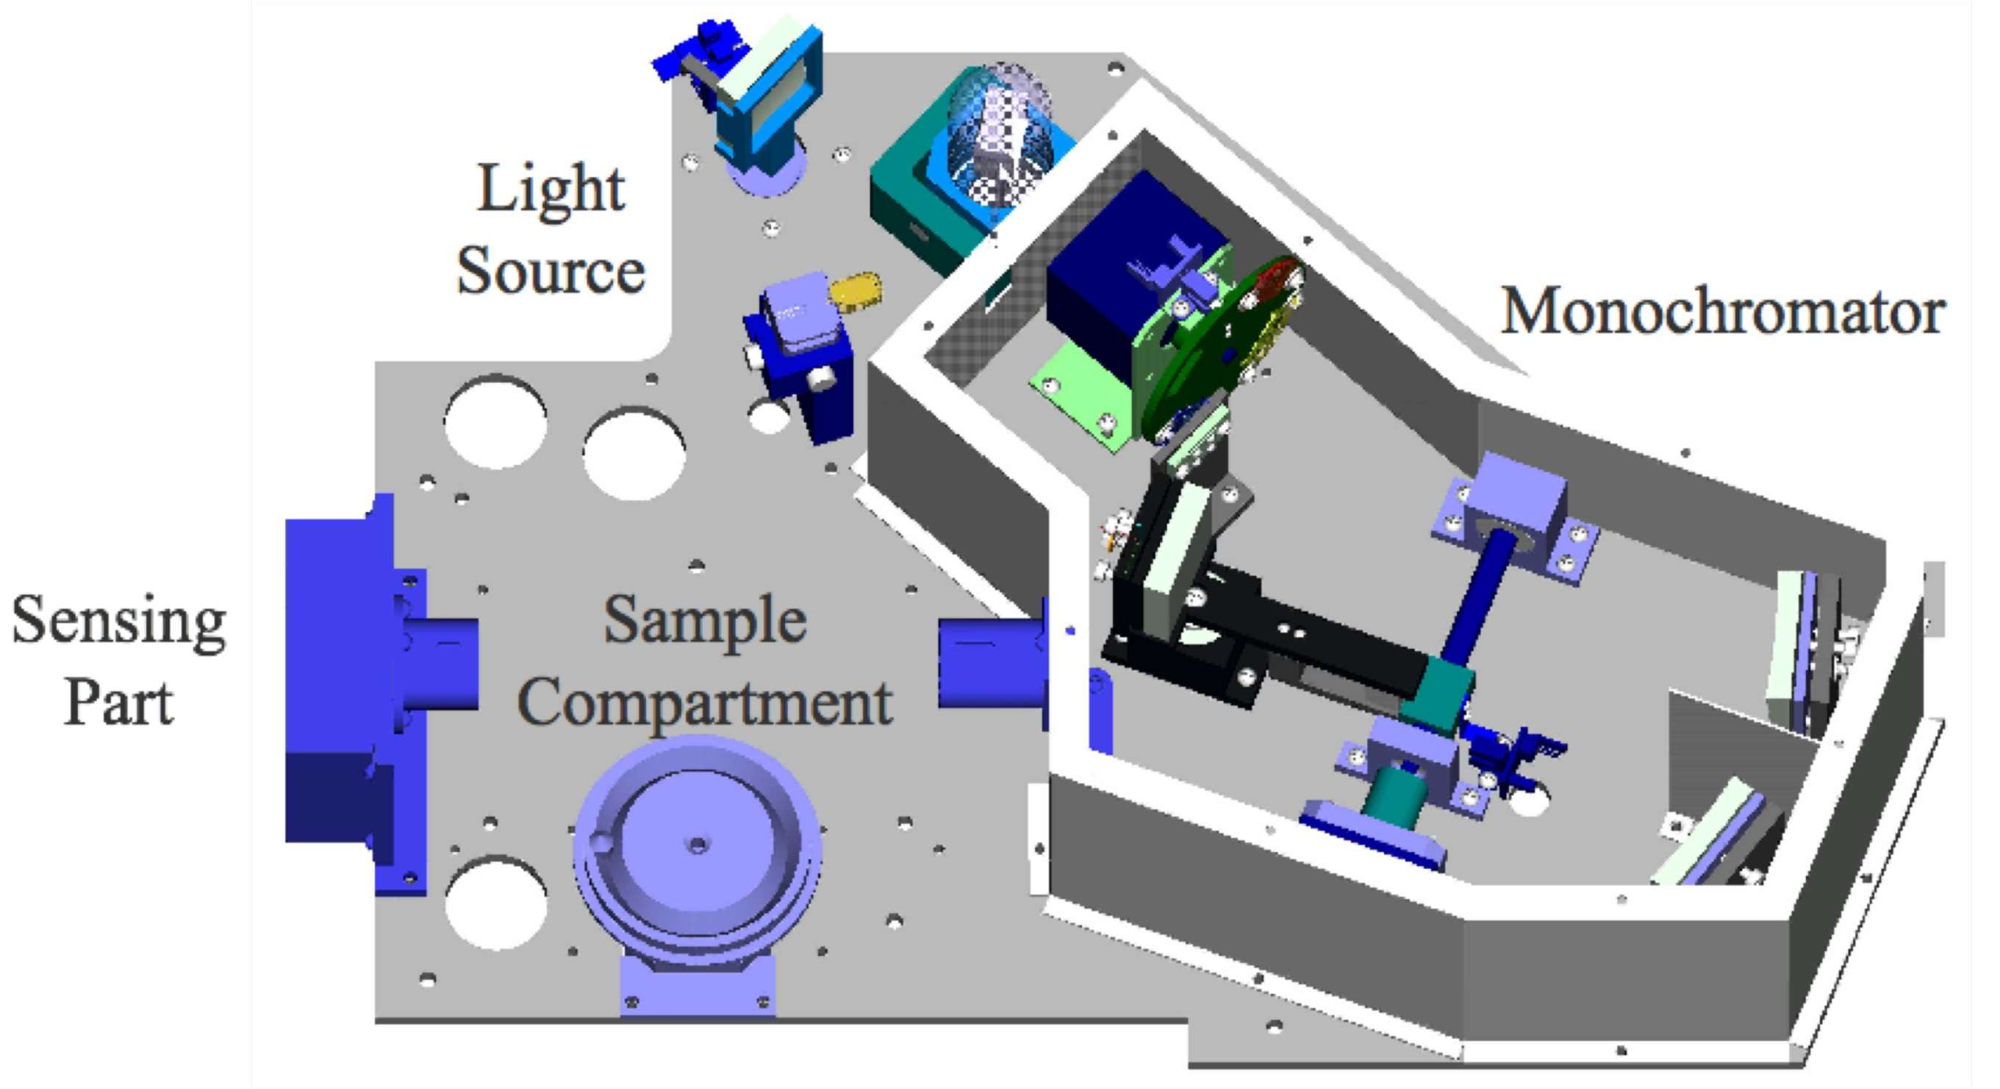
\includegraphics{images/7e7bd118-08b0-4344-a5b9-14ff939eb63e-uschematicdiagramuvvisspectrophotometer.png}}{}
\makeatother 
\caption{{Schematic diagram of a typical UV-Vis spectrophotometer \unskip~\protect\cite{693772:16435037}}}
\label{f-82062f273073}
\end{figure*}
\egroup




\subsection{UV Sources}Open arcs, fluorescent, incandescent, lasers, and LEDs are the typical UV sources. In spectroscopy implementations, the UV source shall be stable (commonly characterized by fluctuation or short-term stability) and with sufficient power intensity (usually quantified by the ratio of variation in the intensity of emitted light to the mean intensity of the emitted light) for the desired wavelength. The short-term stability and power intensity are essential factors in defining the accuracy and reliability of a spectrophotometer\unskip~\cite{693772:16434827}.

Deuterium UV lamps are relatively more stable than other alternatives, due to their extended lifetime and relativity high-intensity light output. However, the major drawbacks of deuterium lamps are the need of a highly stable power supply, and a warm-up time of approximately 30 minutes for thermal equilibrium. Low-pressure mercury lamps are also popular for spectrophotometric sensing of ozone, benzene, toluene, ethyl-benzene, and xylenes as the emission spectrum strongly follows the absorption spectra of these molecules. However, mercury lamps require high power input and has low output stability\unskip~\cite{693772:16434827}. Among the available UV sources, LEDs are an attractive option for future spectrophotometric devices die to portability, low cost, and low power consumption. Different UV sources arer55r5r5 summarized inTable~\ref{tw-b0a1d48481ac}.


\begingroup
\makeatletter\if@twocolumn\@ifundefined{theposttbl}{\gdef\TwoColDocument{true}\onecolumn\onecolumn}{}\fi\makeatother \setlength\LTcapwidth{\textwidth}
\begin{longtable}{p{\dimexpr.14330000000000002\linewidth-2\tabcolsep}p{\dimexpr.25669999999999998\linewidth-2\tabcolsep}p{\dimexpr.20\linewidth-2\tabcolsep}p{\dimexpr.20\linewidth-2\tabcolsep}p{\dimexpr.20\linewidth-2\tabcolsep}}
\caption{{Collation of UV sources for spectrophotometry\unskip~\protect\cite{693772:16434827}.} }
\label{tw-b0a1d48481ac}
\def\arraystretch{1}\\\endfirsthead \hline \noalign{\vskip3pt} \noalign{\textit{Table \thetable\ continued}} \noalign{\vskip3pt} 
\tbltoprule  & \textbf{LED} & \textbf{Deuterium Lamp} & \textbf{Xenon Flash Lamp} & \textbf{Mercury Lamp}\\
\tblmidrule \endhead \hline \noalign{\vskip3pt} \noalign{\textit{\hfill Continued on next page}} \noalign{\vskip3pt} \endfoot \endlastfoot 
\tbltoprule  & \textbf{LED} & \textbf{Deuterium Lamp} & \textbf{Xenon Flash Lamp} & \textbf{Mercury Lamp}\\
\tblmidrule 
\textbf{Wavelength} &
  Single peak &
  Relatively wide spectrum 120{\textendash}400 nm &
  Broad-spectrum 160{\textendash}2000 nm &
  Broad-spectrum 185{\textendash}2000 nm\\
\textbf{Stability of light output} &
  Excellent temporal and spatial stability. &
  Good. \mbox{}\protect\newline Fluctuation {\textless}0.005\% &
  Relatively poor. Fluctuation {\textless}3\% &
  Relatively poor. Fluctuation {\textless}2\%\\
\textbf{Warm-up time} &
  Instantaneous &
  20{\textendash}30 min &
  Instantaneous &
  1{\textendash}15 min\\
\textbf{Life [hrs]} &
  3000{\textendash}10,000 &
  2000{\textendash}4000 &
  400{\textendash}5000 &
  500{\textendash}3000\\
\textbf{Input wattage [W]} &
  DC powered 6{\textendash}10 V &
  5{\textendash}150 &
  2{\textendash}60 &
  5{\textendash}150\\
\textbf{Thermal effect on samples} &
  None &
  Sample can be \mbox{}\protect\newline affected by the heat from the lamp &
  None &
  Sample can be \mbox{}\protect\newline affected by the heat from the lamp\\
\textbf{Cost} &
  Low &
  High &
  High &
  Low\\
\textbf{Drive electronics} &
  Simple &
  Complex &
  Complex &
  Complex\\
\textbf{Safety} &
  Low voltage and cold light source &
  High power supply (Input wattage 5{\textendash}150 W) and hot lamp surface &
  High voltage supply (Input wattage 2{\textendash}300 W): sparking risk &
  High voltage supply (Input \mbox{}\protect\newline wattage 50{\textendash}500 W) and contains mercury in fragile quartz envelop\\
\tblbottomrule 
\end{longtable}
\endgroup
\makeatletter\@ifundefined{TwoColDocument}{}{\twocolumn}\makeatother 




\subsection{UV-LED based spectroscopy}LEDs are semiconductor diodes, which emit light due to the hole-electron interaction, as the energy of an emitted photon depends on the band gap of the semiconductor. LEDs are small and portable with low optical noise, which can be easily incorporated into absorbance measurement detectors. LEDs have lower intensity drifts, low cost, long lifetime (104 h), and low heat generation\unskip~\cite{693772:16434827}. These features made them suitable for low-power portable applications.
    
\section{Paper Review: High power deep UV-LEDs for analytical optical instrumentation \unskip~\protect\cite{693772:16459460}}
LEDs have been implemented as light sources in various applications of optical sensing and chemical analyzes, as they offer a better alternative to traditional light sources (low-cost, small size, robustness, portability, and low noise). However, the lack of rapid, facile and accurate radiometric analysis of LEDs is a major limiting factor which constrains their practical use\unskip~\cite{693772:16434801}.

Li et al. intention was to report the performance of three new deep UV-LEDs (OPTAN255H, OPTAN255J and OPTAN280J), and investigate their feasibility for analytical applications. The LEDs selection was based on the maximum emission wavelength and maximum optical power\unskip~\cite{693772:16459460}.



\subsection{Chemicals and reagents}As stated in Li et al.'s article, chromate in 50 mM NaOH solution was used as absorbing probe. The capillary was firstly flushed with water or the chromate standard solution with approximately 10 capillary volumes, then the flow was stopped and the absorbance was measured under static conditions. Each test solution was measured three times and in increasing concentration. Sodium hydroxide and sodium chromate were purchased from Sigma-Aldrich (St. Louis, MO, USA). The solutions were prepared fresh weekly and stored at 4 \ensuremath{\circ }C when not in use\unskip~\cite{693772:16459460}.



\subsection{Instrumentation \& Method}Li et al. used an USB2000 + XR1-ES miniature fiber optic based spectrometer (OceanOptics, Dunedin, FL, USA) with integration time set at 3 ms to measure the spectra of the deep UV-LEDs. The spectrometer used has a bandwidth of 2 nm. The spectrophotometer and LEDs were mounted into an optical bench (ACH-CUV-VAR, Ocean Optics, Dunedin, FL, USA) without additional optical fibers or lens. The data acquisition and processing of the emission spectra of deep UV-LEDs was processed with SpectraSuite software (Ocean Optics, Dunedin, FL, USA)\unskip~\cite{693772:16459460}. Li et al.'s paper assess the effects of input current and voltage on the intensities of the visible parasitic emission and the desirable UV emission. 



\subsection{Results}



\subsubsection{Emission spectrum}Li et al. experimental results show that while the parasitic emission still exists with the new generation deep UV-LEDs, with increasing input current the ratio of undesirable parasitic emission to the main deep UV emission rapidly decreased to values as low as 0.1\% at the maximum forward current (100 mA) Figure~\ref{f-6a19629c79ef}\unskip~\cite{693772:16459460}.


\bgroup
\fixFloatSize{images/00f20b2f-0b5a-498f-99f8-0f7bd4ddeb7e-uintensityofdeepuvemissionandparasiticemission.png}
\begin{figure*}[!htbp]
\centering \makeatletter\IfFileExists{images/00f20b2f-0b5a-498f-99f8-0f7bd4ddeb7e-uintensityofdeepuvemissionandparasiticemission.png}{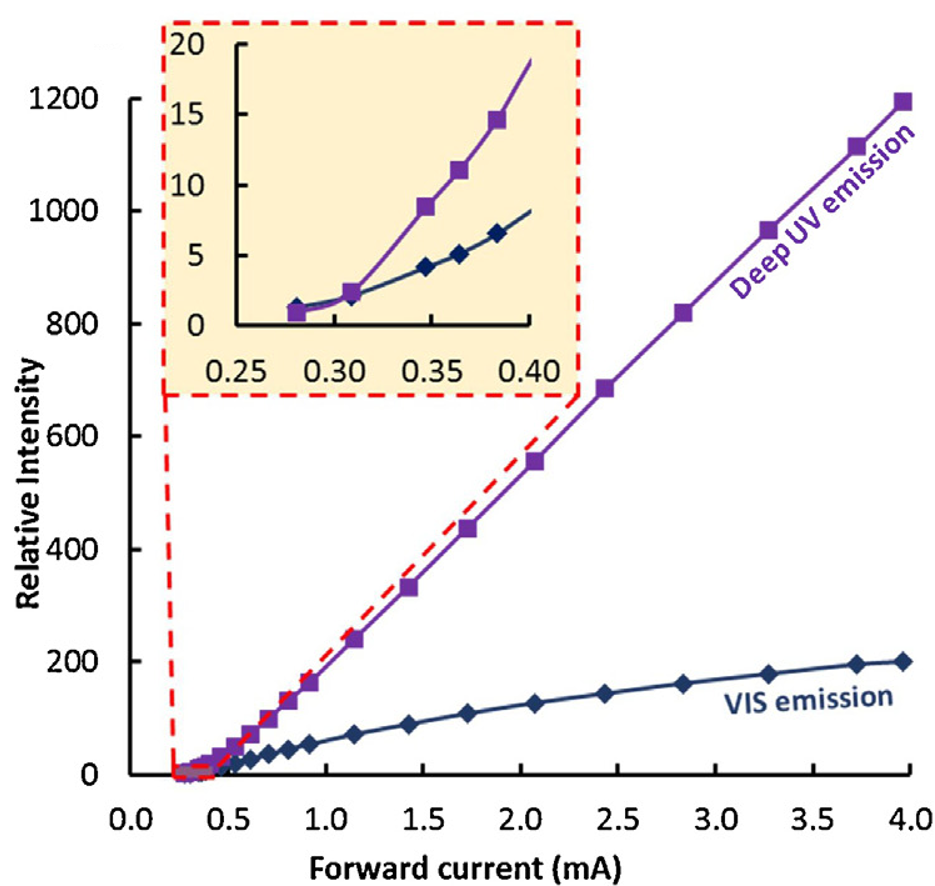
\includegraphics{images/00f20b2f-0b5a-498f-99f8-0f7bd4ddeb7e-uintensityofdeepuvemissionandparasiticemission.png}}{}
\makeatother 
\caption{{The intensity of deep UV emission and parasitic emission at different forward currents. The plots show unequal increasing rate of deep UV emission and the parasitic Vis emission\unskip~\protect\cite{693772:16459460}.}}
\label{f-6a19629c79ef}
\end{figure*}
\egroup
Since the forward current increases, the parasitic emission becomes saturated while the deep UV emission increases linearly, resulting to extremely low P/DUV ratio at its maximum forward current Figure~\ref{f-23bca4aac565}, which overcomes the parasitic emission issue\unskip~\cite{693772:16459460}.


\bgroup
\fixFloatSize{images/35099b97-39f6-4470-8f92-209c7f283a99-uemissionspectraofnewgenerationoptan255h.png}
\begin{figure*}[!htbp]
\centering \makeatletter\IfFileExists{images/35099b97-39f6-4470-8f92-209c7f283a99-uemissionspectraofnewgenerationoptan255h.png}{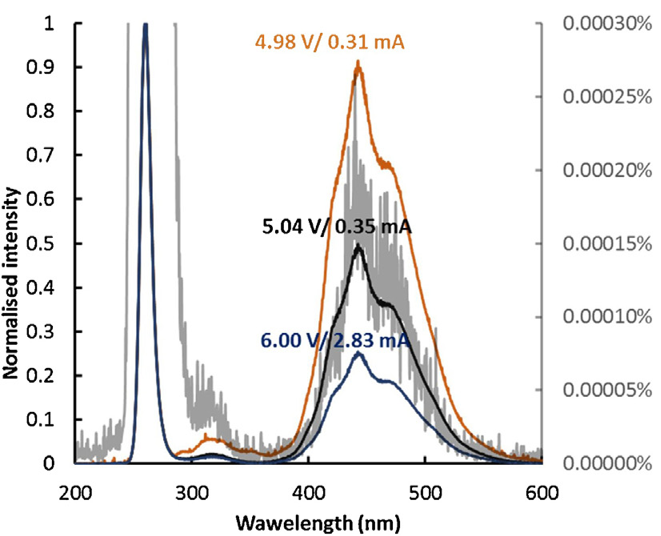
\includegraphics{images/35099b97-39f6-4470-8f92-209c7f283a99-uemissionspectraofnewgenerationoptan255h.png}}{}
\makeatother 
\caption{{The emission spectra of new generation deep UV-LED (OPTAN255H) at 3 selected input currents (left axis) and at the maximum current (100 mA, grey line, right axis). The parasitic emission became relatively lower with increasing forward current and at the maximum forward current (100 mA) the parasitic emission is only about 2 \ensuremath{\times} 10-4\% (right axis) \unskip~\protect\cite{693772:16459460}}}
\label{f-23bca4aac565}
\end{figure*}
\egroup
Li et al. susoect that the parasitic emission can originate either in the presence of undesirable bands of lower energy in the emitting semiconductor, or by the presence of materials in the LED that exhibit fluorescence or phosphorescence behaviors\unskip~\cite{693772:16459460}.



\subsubsection{Detection performance and demonstration in capillary chromatography}Li et al. implemented a new generation deep UV-LED (255 nm) as light source for a photometric on capillary detection, showing excellent linearity with stray light down to 0.8\%, and effective path length above 92\% of the used capillary inner diameter, and finally the performance was demonstrated by detecting four parabens separated by miniaturized capillary liquid chromatography Figure~\ref{f-69d087c4c664}\unskip~\cite{693772:16459460}.


\bgroup
\fixFloatSize{images/3af05996-142a-4ae0-987e-11cce33c727b-uisocraticseparationofparabensofdifferentconcentrations.png}
\begin{figure*}[!htbp]
\centering \makeatletter\IfFileExists{images/3af05996-142a-4ae0-987e-11cce33c727b-uisocraticseparationofparabensofdifferentconcentrations.png}{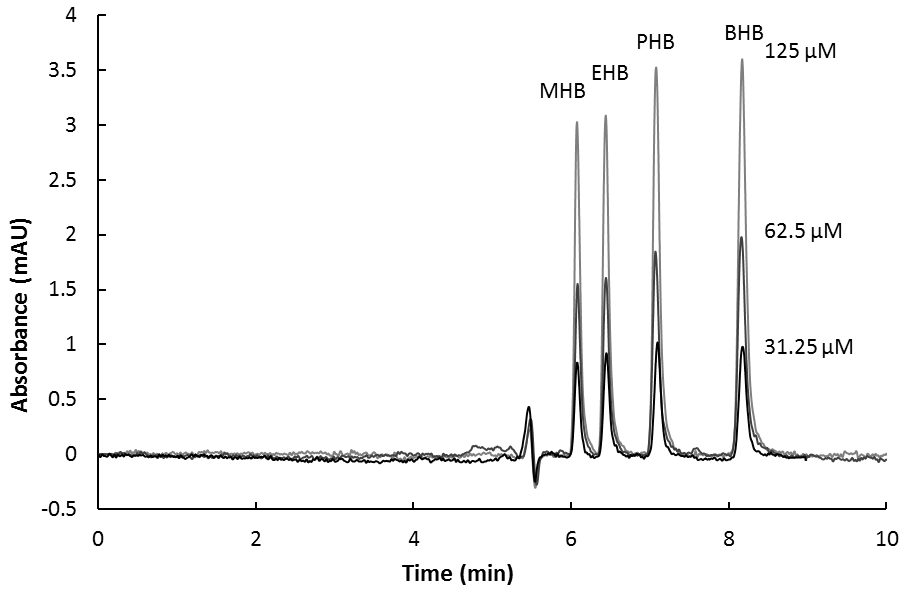
\includegraphics{images/3af05996-142a-4ae0-987e-11cce33c727b-uisocraticseparationofparabensofdifferentconcentrations.png}}{}
\makeatother 
\caption{{Isocratic separation of parabens of different concentrations. Conditions: Concentration of all analytes in three separations was 31.25 \ensuremath{\mu}M, 62.5 \ensuremath{\mu}M or 125 \ensuremath{\mu}M. methyl 4-hydroxybenzoate(MHP), ethyl 4-hydroxybenzoate (EHB), mM propyl 4-hydroxybenzoate (PHB), and butyl 4-hydroxybenzoate (BHB); Solvent: 50 mM ammonium acetate -acetonitrile 50/50 (v/v); flow rate: 0.5 mL min\ensuremath{^{-1}}; detection: 255 nm LED on-capillary photometric detector. Deep UV-LED forward current 100 mA\unskip~\protect\cite{693772:16459460}.}}
\label{f-69d087c4c664}
\end{figure*}
\egroup
The measurement reproducibility is within 1{\textendash}3\% relative standard deviation. Due to the high optical intensity of the new generation deep UV-LED, the baseline noise was low, determined as only 13.4 \ensuremath{\mu}AU, which is approximately 10 times lower than baseline noise for the same on-capillary detector using the old generation deep UV-LEDs. The on-capillary detector using the new generation deep UV-LED also offered excellent linearity. The detection performance comparison of a same on-capillary detector using old generation and new generation deep UV-LED as light source is shown inTable~\ref{tw-10fa7620e2c2}.


\begin{table*}[!htbp]
\caption{{Comparison of the detection performance of on-capillary detector using old generation and new generation deep UV-LED as light source\unskip~\protect\cite{693772:16459460}.} }
\label{tw-10fa7620e2c2}
\def\arraystretch{1}
\ignorespaces 
\centering 
\begin{tabulary}{\linewidth}{LLLLL}
\tbltoprule Generation of deep UV-LEDs & Stray light & Baseline noise [\ensuremath{\mu}AU] & Measured effective pathlength [percentage of the capillary ID] & Upper LOD linearity (mAU)\\
\tblmidrule 
Old (sapphire substrate based) &
  30.5\% &
  100 &
  79\% &
  31\\
New (AIN substrate based) &
  0.8\% &
  13.4 &
  95\% &
  745\\
\tblbottomrule 
\end{tabulary}\par 
\end{table*}
\clearpage 
    

\bibliographystyle{blank}

\bibliography{\jobname}

\section*{Author biography}

\bioItem[images/bf0f1284-fa36-4678-a9e7-05671376e50c-umeitesm]{Antonio Osamu Katagiri Tanaka}{ .

MNT16

A01212611}
\printBio 

\end{document}
